%%%%%%
%
% $Author: Abishek $
% $Date: 06.05.2024 $
% $Path: BA24-02-Time-Series\report\Contents\en$
% $Version: 1.0 $
%
%
% !TeX encoding = utf8
% !TeX root = Rename
% !TeX TXS-program:bibliography = txs:///bibtex

\chapter{Machine Learning Pipeline}

In this chapter, we delve into the intricate process of developing a machine learning pipeline for forecasting air quality parameters. We will explore the structure, idea formulation, flow chart representation, and the detailed steps involved in constructing a robust machine learning (ML) pipeline specifically designed for air quality forecasting.
\section{Structure} 
Machine learning plays a pivotal role in forecasting air quality, leveraging data-driven insights and sophisticated algorithms to predict pollutant concentrations and support decision-making in urban environments. Understanding the fundamentals of machine learning is crucial for developing accurate and efficient forecasting models in this domain \cite{Fan:2019}.The development of an air quality forecasting system involves several key steps 
\subsection {Data Collection}
 Gather comprehensive air quality data including pollutant concentrations (NO2, SO2, CO, O3) and meteorological parameters (temperature, humidity) from monitoring stations and weather APIs.\cite{Fan:2019}
\subsection {Data Preprocessing}
Clean and preprocess data by handling missing values, scaling features, and encoding categorical variables. This ensures data quality and prepares it for model training \cite{GeeksforGeeks:2024}.
\subsection {Model Development}
 Choose suitable algorithms such as regression models, ensemble methods, or neural networks based on the forecasting task (e.g., predicting pollutant levels over time).Train the selected model on a training dataset to learn patterns and relationships between pollutants and meteorological factors. Utilize techniques like gradient descent for optimization\cite{GeeksforGeeks:2024}.
\subsection {Model Evaluation}
Assess model accuracy using metrics like Mean Absolute Error (MAE), Root Mean Squared Error (RMSE), and R-squared (R2) for regression tasks, ensuring the model's ability to generalize to unseen data\cite{GeeksforGeeks:2024}.
\subsection {Deployment}
Fine-tune model hyperparameters using techniques like grid search or randomized search to enhance predictive performance and robustness.Integrate the trained model into a production environment for real-time air quality forecasting. Ensure scalability and reliability using containerization tools like Docker\cite{GeeksforGeeks:2024}.
\section{Idea}
The core idea is to use historical air quality and meteorological data to predict future air quality levels. Combining historical data with recent data from on-ground sensors to create predictive models helps in forecasting air pollution. Machine learning approaches have shown promise over traditional time series forecasting methods due to their ability to handle complex relationships between pollutants and meteorological conditions. This involves:

\begin{itemize}
	\item \textbf{Concept:} Utilizing ML algorithms to analyze patterns in historical data and make future predictions.
    \item \textbf{Hypothesis:} Factors such as temperature, humidity, wind speed, and traffic volume significantly influence air quality.
    \item \textbf{Expected Outcome:} Achieving high accuracy in predictions to inform the public and assist policymakers in taking preemptive measures.
\end{itemize}





\section{ML Pipeline}
	A Machine Learning (ML) Pipeline refers to a systematic process or workflow\ref{fig:ml_pipeline} that integrates various stages of machine learning model development, from data collection and preprocessing to model training, evaluation, and deployment. The primary goal of an ML pipeline is to automate and streamline the process of building, testing, and deploying machine learning models efficiently.\cite{Ravindiran:2023}

	\subsection{Air Quality Dataset}
	 This is the starting point, representing the raw dataset that contains various factors (features) related to air quality such as pollutant levels, weather conditions, geographical data, etc.
	
	\subsection{Data Preprocessing}
     Prepares the dataset for analysis and modeling by ensuring data quality and consistency.
	\begin{itemize}
		\item \textbf{Check Missing Values:} Identifies and handles missing data points.
		\item \textbf{Remove Instances:} Deletes rows with missing data that cannot be imputed or interpolated.
	\end{itemize}
	
	\subsection{Exploratory Data Analysis (EDA)}
	 Investigates the dataset to summarize its main characteristics, often using statistical graphics and other data visualization methods.
	\begin{itemize}
		\item \textbf{Identify Features:} Determines which variables (features) are most likely to influence air quality predictions.
		\item \textbf{Statistical Analysis:} Uses statistical methods to understand the relationships between variables and their impact on air quality.
		\item \textbf{Data Visualization:} Creates visual representations (charts, graphs) to explore data patterns and distributions.
	\end{itemize}
	
	\subsection{Data Normalization}
	Adjusts the data to have a common scale without distorting differences in the ranges of values, which can improve the performance and convergence of machine learning algorithms.
	\begin{itemize}
		\item \textbf{Square Root Transformation:} One method of transforming skewed data distributions to approximate a normal distribution.
	\end{itemize}
	
	\subsection{Machine Learning Regression Model}
	 Develops a predictive model that can estimate the Air Quality Index (AQI) based on the dataset.
	\begin{itemize}
		\item \textbf{Dataset Split (Train/Test):} Divides the dataset into training and testing sets to evaluate the model's performance.
		\item \textbf{Train Model:} Utilizes the training data to teach the machine learning model the patterns in the dataset.
		\item \textbf{Air Quality Prediction Model \& Validation:} Validates the trained model's accuracy and reliability using the test data set aside during training.
	\end{itemize}
	
	\subsection{Deployment (Target - Predictions)}
     Uses the trained and validated model to predict the AQI values for new data inputs, completing the workflow and achieving the goal of predicting air quality\cite{Ravindiran:2023}.
	

	\section{Air Quality Prediction Workflow}
	\tikzstyle{startstop} = [rectangle, rounded corners, minimum width=3cm, minimum height=1cm,text centered, draw=black, fill=blue!30]
	\tikzstyle{process} = [rectangle, minimum width=3cm, minimum height=1cm, text centered, draw=black, fill=orange!30, align=center]
	\tikzstyle{arrow} = [thick,->,>=stealth]
	
	\begin{figure}[h]
		\centering
		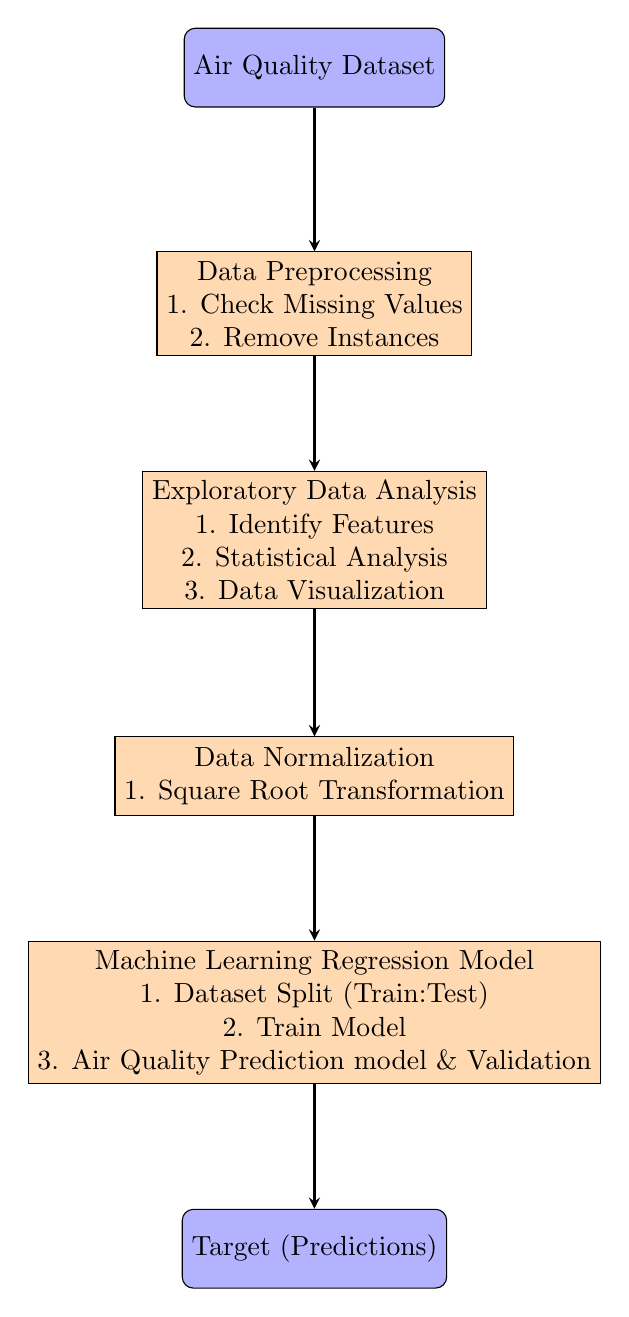
\begin{tikzpicture}[node distance=3cm]
			
			
			\node (dataset) [startstop] {Air Quality Dataset};
			\node (preprocess) [process, below of=dataset] {
				Data Preprocessing \\
				1. Check Missing Values \\
				2. Remove Instances
			};
			\node (eda) [process, below of=preprocess] {
				Exploratory Data Analysis \\
				1. Identify Features \\
				2. Statistical Analysis \\
				3. Data Visualization
			};
			\node (normalize) [process, below of=eda] {
				Data Normalization \\
				1. Square Root Transformation
			};
			\node (mlmodel) [process, below of=normalize] {
				Machine Learning Regression Model \\
				1. Dataset Split (Train:Test) \\
				2. Train Model \\
				3. Air Quality Prediction model \& Validation
			};
			\node (deploy) [startstop, below of=mlmodel] {Target (Predictions)};
			
			
			\draw [arrow] (dataset) -- (preprocess);
			\draw [arrow] (preprocess) -- (eda);
			\draw [arrow] (eda) -- (normalize);
			\draw [arrow] (normalize) -- (mlmodel);
			\draw [arrow] (mlmodel) -- (deploy);
			
		\end{tikzpicture}
		\caption{Machine Learning Pipeline for Air Quality Forecasting}
		\label{fig:ml_pipeline}
	\end{figure}
	
	\subsection{Flow of the Process}
\textbf{Sequential Approach:} The flowchart demonstrates a structured approach from data preprocessing through exploratory analysis, normalization, model building, validation, and finally, deployment of the predictive model.

\textbf{Iterative Refinement:} Throughout the process, adjustments and refinements are made based on insights gained from the data exploration and model evaluation stages, ensuring that the model is accurate and robust\cite{Ravindiran:2023}.

